% This is samplepaper.tex, a sample chapter demonstrating the
% LLNCS macro package for Springer Computer Science proceedings;
% Version 2.20 of 2017/10/04
%
\documentclass[runningheads]{llncs}
%
\usepackage[utf8x]{inputenc} %Para las tildes
\usepackage{graphicx}
\usepackage[spanish, es-tabla]{babel}
\usepackage[T1]{fontenc}

% Used for displaying a sample figure. If possible, figure files should
% be included in EPS format.
%
% If you use the hyperref package, please uncomment the following line
% to display URLs in blue roman font according to Springer's eBook style:
% \renewcommand\UrlFont{\color{blue}\rmfamily}

\begin{document}
%

\title{Control de temperatura para el estudio del voltaje de ruptura de SiPMs}
%
%\titlerunning{Abbreviated paper title}
% If the paper title is too long for the running head, you can set
% an abbreviated paper title here
%
\author{J. Sánchez Villafrades\inst{1}\orcidID{0000-0002-2338-3425},\\
J. Peña Rodríguez\inst{2}\orcidID{0000-0002-9861-1023},\\
L.A. Nunez \inst{2}\orcidID{0000-0003-4575-5899},\\
R. Calderón Ardila \inst{2}\orcidID{0000-0002-3129-9100}
}
%
\authorrunning{J. Sánchez et al.}
% First names are abbreviated in the running head.
% If there are more than two authors, 'et al.' is used.
%
\institute{Escuela de Ingeniería Eléctrica Electrónica y de Telecomunicaciones, Universidad Industrial de Santander, Bucaramanga 680002, Colombia 
\email{juan.sanchez7@correo.uis.edu.co} \and
Escuela de Física , Universidad Industrial de Santander,  Bucaramanga 680002, Colombia}
%\email{jesus.peña@correo.uis.edu.co} \and
%Escuela de Física , Universidad Industrial de Santander,  Bucaramanga 680002, Colombia
%\email{lnuñes@uis.edu.co}


\maketitle              % typeset the header of the contribution
%
\begin{abstract}
En este trabajo se presenta el modelado, sintonización e implementación de un sistema de control de temperatura del tipo Proporcional Integral Derivativo (PID) que, haciendo uso de dispositivos Peltier, genera un ambiente de temperatura controlada. Este sistema se utilizó para caracterizar los principales parámetros de funcionamiento de SiPM. En este caso, se estima el voltaje de ruptura de los SiPM S13360-1350CS mediante las curvas de corriente-voltaje obtenidas en condiciones de oscuridad en el rango de temperatura  0 a 50$^{\circ}$ C.\\ %Más específicamente se estudió el SiPM S13360-1350CS, fabricado por HAMAMATSU, con un tamaño de píxel de 50 x 50 $\mu m^{2}$ y un área fotosensible de $1.3~x~1.3~mm^{2}$.\\%También Se midió las características de corriente-voltaje en condiciones de oscuridad y se calculó su dependencia de la temperatura.\\


{\bf Palabras clave:} Controlador PID $\cdot$ Dispositivo Peltier $\cdot$ Fotomultiplicadores de Silicio $\cdot$ Voltaje de ruptura.
\end{abstract}
%
%
%
\section{Introducción}
Los fotomultiplicadores de silicio (SiPMs, por sus siglas en inglés), son actualmente una alternativa a los detectores de fotones tradicionales, como los tubos fotomultiplicadores~\cite{Intro_SIPM_Sensl}. Estos están conformados por una matriz de fotodiodos de avalancha operando en modo Geiger~\cite{Sipm_S13360_1350CS_datasheet}. Los SiPM son compactos, tienen una rápida respuesta, alta ganancia y bajo voltaje de operación; de ahí que, son muy utilizados en los campos de imágenes médicas, biofotónica, LiDAR y física de altas energías (e.g. detectores de centelleo )~\cite{study_break_voltage_SIPM,Break_voltage_dif_temp_SIPM}. Sin embargo, los SiPM son sensibles a cambios de temperatura~\cite{Intro_SIPM_Sensl}.\\ \\
Actualmente, el Grupo de Investigación en Relatividad y Gravitación (GIRG) y el Grupo Halley de la Universidad Industrial de Santander están desarrollando el Telescopio de Muones (MuTe), el cual será instalado en el volcán  Cerro Machín (Tolima, Colombia)~\cite{Mute_oficial}. MuTe está conformado por un hodoscopio de barras centelladoras, en cuyos extremos están instalados SiPMs que se encargan de detectar los fotones generados durante el proceso de centelleo. En el sitio de detección la temperatura varia de 8 a 25 $^{\circ} C$ debido a las condiciones climáticas ~\cite{temp_machin}, por lo tanto se hace necesario conocer el efecto de esta variación en el desempeño de los SiPMs. El voltaje de ruptura es el principal parámetro de funcionamiento de los SiPMs, ya que determina el voltaje de polarización. Considerando  que en las hojas de datos el fabricante solo se especifica su valor a temperatura ambiente, se hace necesario caracterizar este parámetro para el rango de temperatura al cual será expuesto el detector.\\ \\% para esto se diseñó un sistema de control de temperatura de tipo PID.\\ \\
Teniendo en cuenta los aspectos anteriormente mencionados, en este trabajo se presenta el diseño de un sistema de control de temperatura de tipo PID para la parametrización de los SiPM. En primer lugar, se explica el principio de funcionamiento de los dispositivos Peltier que se emplean en el sistema de control para realizar el calentamiento y la refrigeración del SiPM. Además se expone el sistema de primer orden con tiempo muerto (FOPDT) utilizado como modelo del sistema térmico, la sintonización del controlador PID y las características del SiPM estudiado. En segundo lugar, se plantea la configuración experimental utilizada para el sistema de control de temperatura. En el capítulo cuatro, se muestran los modelos obtenidos para el sistema de control temperatura, la respuesta del sistema cuando se implementa el controlador PID y el comportamiento del voltaje de ruptura en función de la temperatura. Finalmente, se exponen los principales resultados tanto del sistema de control de temperatura, como de la caracterización del voltaje de ruptura.\\
\section{Metodología}
Para el estudio del voltaje de ruptura de los SiPM S13360-1350CS de Hamamatsu es necesario obtener la curva característica corriente-vs-voltaje para varias temperaturas, por lo tanto se diseña un sistema de control de temperatura basado en dispositivos Peltier~\cite{peltier_physical_principles}, que permite el calentamiento y la refrigeración del interior de una caja, donde se ubica el SiPM para su caracterización. El controlador PID se basa en el modelo FOPDT de la planta (\textit{Puente H}, Dispositivos Peltier y sensor de temperatura). Por otra parte, para realizar la conversión de la corriente oscura del SiPM a voltaje fue necesario utilizar un amplificador de transimpedancia (TIA). 
\subsection{Dispositivo Peltier} 
El efecto Peltier fue descubierto en 1834 por el físico francés Jean Charles Athanase Peltier,~\cite{peltier_theory}. Los dispositivos Peltier consisten en un arreglo de  semiconductores (tipo-n y tipo-p) unidos por una placa metálica que conforma un área de contacto  que absorbe o produce calor cuando una corriente eléctrica fluye a través de ella. Así pues, la dirección de la corriente eléctrica determina si el área se calienta o se enfría~\cite{peltier_physical_principles,Peltier_SIPM}. 
El calor generado mediante este efecto por unidad de tiempo esta determinado por:%\ref{peltier_eq}.
\begin{equation}
Q_{Pe}=(\Pi_{A}-\Pi_{B})\cdot I
\label{peltier_eq}
\end{equation}
donde $\Pi_{(A,B)}$ son los coeficientes Peltier de cada semiconductor e $I$ es la corriente eléctrica.\\
En este caso, para diseñar un sistema de control de temperatura que funcione en el rango de $0-50~^\circ C$ se utilizó un dispositivo Peltier para calentar o refrigerar la superficie que está en contacto con el SiPM. 

\subsection{Sistema FOPDT}
Un FOPDT ( First Order Plus Dead Time) es un modelo dinámico ampliamente utilizado para la obtención de los parámetros de sintonización de un controlador PID~\cite{FOPDT}, su función de transferencia está dada por:
\begin{equation}
Gp(s)=  \frac{k\cdot e^{-Ls}}{1+Ts}
\end{equation}
donde $k$ es la ganancia en estado estable de la planta, $T > 0$  representa la constante de tiempo de la planta y $L > 0$ es el tiempo muerto. Para la identificación de estos parámetros existen varios procedimientos, uno de estos es de forma gráfica y otro (el que se utilizó en este trabajo) mediante un algoritmo de optimización que ajusta los parámetros $k$, $T$ y $L$ a los datos.  

\subsection{Controlador PID}
Para mantener estable la temperatura del SiPM es necesario implementar un controlador PID digital,  con periodos de muestreo discretos y con una versión filtrada del término derivativo~\cite{Astrom_control_PID}, donde se remplaza la derivada del error por la derivada de la señal de entrada (ver Ec.~\ref{pid_eq}).%que permita  que la temperatura se establezca en el menor tiempo posible y sin oscilaciones 
\begin{equation}
u(t)=u_{bias} + k_{p}\cdot e(t) + k_{i}\cdot \displaystyle\sum_{i=1}^{n_{t}} e_{i}(t)\cdot \Delta_{t} - k_{d}\cdot \frac{y_{n_{t}}-y_{n_{t-1}}}{\Delta_{t}}  
\label{pid_eq}
\end{equation}
En la Fig.~\ref{Diag_PID} se muestra un diagrama simplificado de nuestro sistema de control. El controlador (PID) se implementó en un microcontrolador Arduino Uno, en este caso, la planta se compone de los dispositivos Peltier y el puente H y el lazo de realimentación es un sensor de temperatura.  
\begin{figure}[ht]
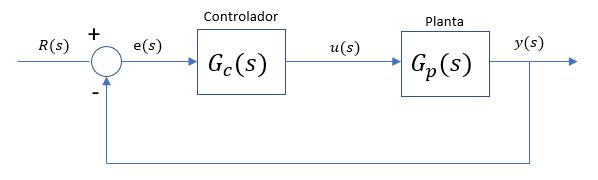
\includegraphics[width=0.7\textwidth]{diagrama_control.JPG}
\centering
\caption{Sistema de control realimentado con ganancia unitaria.} 
\label{Diag_PID}
\end{figure}

\subsection{Sensor Estudiado: SiPM S13360-1350CS}
% El SIPM estudiado es desarrollado por HAMAMATSU 
El SiPM es un dispositivo opto-semiconductor de precisión, utilizado para el conteo de fotones~\cite{Intro_SIPM_Sensl} que consiste en múltiples píxeles APD (fotodiodos de avalancha) operando en modo Geiger~\cite{Sipm_S13360_1350CS_datasheet,Apd_Hamamatsu}. Los SiPM operan con bajo voltaje ($\sim 60V$),  tienen alta ganancia ($10^{6}$), alta eficiencia de detección, respuesta rápida y son inmunes a campos magnéticos, por lo que son un potencial reemplazo de los detectores convencionales como los tubos fotomultiplicodores (PMT)~\cite{Measuring_MPPC}.\\ \\
En este caso, el SiPM que se estudió es el S13360-1350CS de Hamamatsu, el cual tiene un tamaño de píxel de $50~\times~50~\mu m^{2}$, un área foto sensible de $1.3~\times~1.3~mm^{2}$ y cuenta con 667 píxeles~\cite{Apd_Hamamatsu}. 

\section{Configuración experimental}
El estudio del voltaje de ruptura del SiPM se realizó bajo condiciones de temperatura controlada, en el rango de $ 0 $ a $50~^\circ C$, utilizando dos celdas Peltier (TEC1-12706)~\cite{datasheet_Peltier} y una caja de aluminio recubierta con un aislante térmico, como se muestra en la Fig.~\ref{Sistema_experimental}. La caja oscura y las celdas Peltier están unidas mediante una pasta térmica. El SiPM se ubicó dentro de la caja junto con un sensor de temperatura LM35, como  se muestra en la Fig.~\ref{caja}. Este sensor se utilizó para monitorear la temperatura dentro de la cámara y, a su vez, realizar la realimentación del sistema de control PID. El algoritmo de control se implementó en un microcontrolador Arduino Uno, el cual realiza la acción de control mediante una señal PWM que es convertida en una corriente proporcional al ciclo útil de dicha señal a través de un puente H (\textit{driver}) como se muestra en la Fig.~\ref{sistema_termico}.

\begin{figure}[ht]
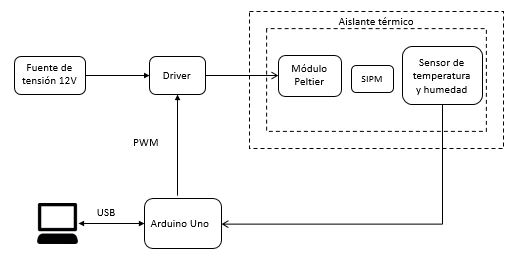
\includegraphics[width=0.7\textwidth]{Diagrama_Camara.JPG}
\centering
\caption{Diagrama de bloques del sistema de control de temperatura.} 
\label{sistema_termico}
\end{figure}

Utilizando la configuración descrita anteriormente se estudia el desempeño en DC del SiPM. Durante las mediciones el SiPM está conectado a un módulo C11204-01 de Hamamatsu que permite controlar su voltaje de polarización~\cite{fuente_hamamatsu}, así como al circuito que realiza la medición de su corriente. Estas mediciones se realizan en condiciones de oscuridad a diferentes temperaturas para obtener las curvas IV (corriente-vs-voltaje) características del SiPM. 

\begin{figure}[ht]
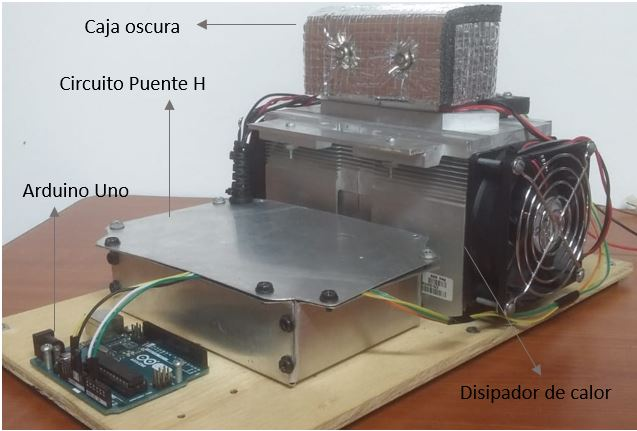
\includegraphics[width=0.7\textwidth]{Sistema_termico.JPG}
\centering
\caption{Sistema de control de temperatura.} 
\label{Sistema_experimental}
\end{figure}

\begin{figure}[ht]
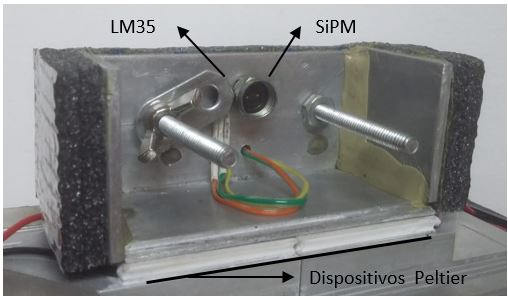
\includegraphics[width=0.7\textwidth]{caja.JPG}
\centering
\caption{Configuración interna de la caja oscura donde se puede observar la ubicación del SiPM, del sensor de temperatura LM35 y los dispositivos Peltier.} 
\label{caja}
\end{figure}
\section{Resultados}
\subsection{Modelado del sistema térmico}
El modelo dinámico del sistema térmico se obtuvo basándonos en el modelado de \textit{caja negra}, el cual es usado cuando no se conocen todos los parámetros físicos del sistema. Dicho método consiste en observar la salida del sistema cuando se estimula con una señal conocida. En este caso, la entrada es una señal PWM con un ciclo útil determinado, y la salida es la temperatura medida dentro de la cámara.  

\begin{figure}[ht!]
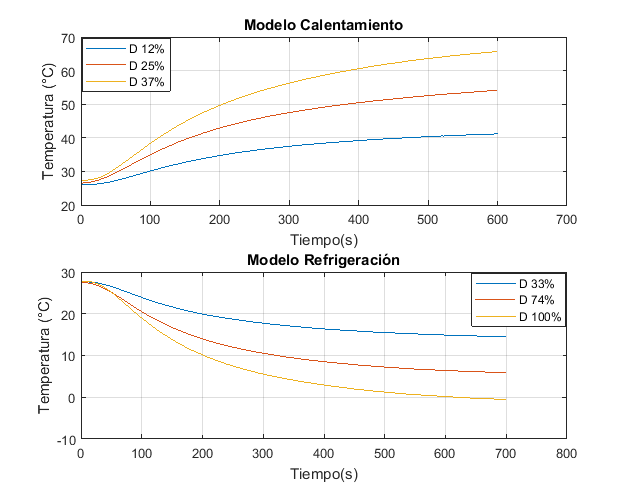
\includegraphics[width=0.8\textwidth]{Modelos.png}
\centering
\caption{Respuesta del sistema de control térmico. Temperatura de calentamiento para un ciclo útil de $12\%$ (línea azul), $25\%$ (línea roja) y $37\%$ (línea amarilla) (Parte superior). Temperatura de refrigeración para un ciclo útil de $33\%$ (línea azul), $74\%$ (línea roja) y $100\%$ (línea amarilla) (Parte inferior).} 
\label{model_sistema}
\end{figure}
Para la refrigeración se estimuló el sistema con una señal PWM con tres ciclos útiles (D) de $33\%,~74\%~y~100\%$. Para el calentamiento los ciclos útiles fueron de $12\%,~25\%~y~37\%$. Nótese que para el calentamiento no se utilizó el máximo ciclo útil debido a que su efecto sobre el sistema es mucho más agresivo.\\ \\
Con los datos de entrada y salida del sistema, y la herramienta \textit{System Identification} de Matlab, se encontró el modelo FOPDT para el calentamiento (Ec.~\ref{modelo_calentamiento}) y la refrigeración (Ec.~\ref{modelo_refrigeracion}).\\ \\

\begin{equation}
G_{p1}(s)=  \frac{0.46 \cdot e^{-27.38s}}{1+222.52s}
\label{modelo_calentamiento}
\end{equation}

\begin{equation}
G_{p2}(s)=  \frac{-0.12 \cdot e^{-31.96s}}{1+185.81s}
\label{modelo_refrigeracion}
\end{equation}
\subsection{Sintonización del controlador PID}
Con los parámetros $k,~L~y~T$ de los modelos dinámicos del sistema (Ec.~\ref{modelo_calentamiento},~\ref{modelo_refrigeracion}), se utilizó la \textit{PID Tuner toolbox} de Matlab para sintonizar los controladores PID para los sistemas de calentamiento ($k_{p}=11.058;~k_{i}=0.044;~k_{d}=41.45$) y refrigeración ($k_{p}=-30.36;~k_{i}=-0.148;~k_{d}=-100$). El sistema de control se probó con tres temperaturas objetivo, tanto para el calentamiento como para la refrigeración durante 10 minutos (Fig.~\ref{Respuesta_PID}).

\begin{figure}[ht!]
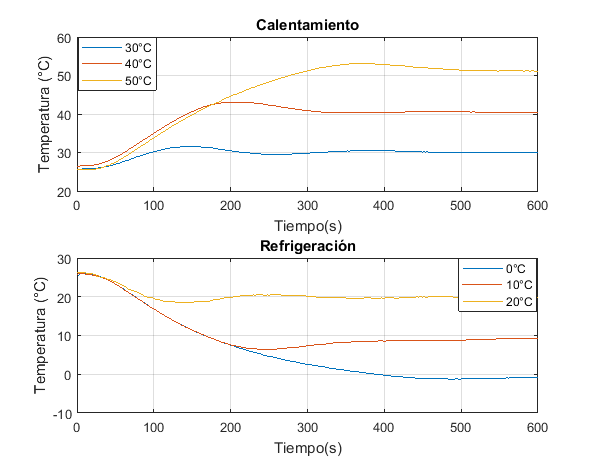
\includegraphics[width=0.8\textwidth]{RespuestaPID.png}
\centering
\caption{Respuesta del sistema de control PID en lazo cerrado. Calentamiento (parte superior) para una temperatura objetivo de $30~^\circ C$ (línea azul), $40~^\circ C$ (línea roja) y $50~^\circ C$ (línea amarilla). Refrigeración para una temperatura objetivo de $0~^\circ C$ (línea azul), $10~^\circ C$ (línea roja) y $20~^\circ C$ (línea amarilla).} 
\label{Respuesta_PID}
\end{figure}

\subsection{Voltaje de ruptura}
El voltaje de ruptura se define como el punto en que el SiPM entra en la zona de amplificación (Región de Avalancha).\\
En la Fig.~\ref{dark_current} se muestra la corriente oscura de el SiPM S13360-1350CS para diferentes voltajes de polarización en un rango de 40-60~V con un paso de 0.5 V. Estas mediciones se realizaron para cuatro temperaturas diferentes (0 $^\circ C$, 10 $^\circ C$, 20 $^\circ C$ y 30 $^\circ C$). Se observó que la pendiente de la curva aumenta en proporción al aumento de la temperatura, esto hace que incremente el voltaje de ruptura.  
%La determinación del voltaje de ruptura se realiza a partir de la medición de la corriente oscura del SIPM en función del voltaje de polarización (~40-60~V), como se muestra en la Fig.~\ref{dark_current}.\\
\begin{figure}[ht!]
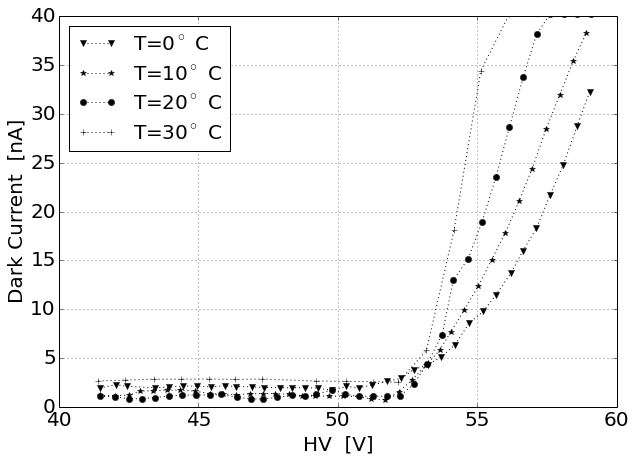
\includegraphics[width=0.7\textwidth]{SiPM_Temp.png}
\centering
\caption{Corriente oscura del SiPM en función del voltaje de polarización para 0 $^\circ C$ (triángulos), 10 $^\circ C$ (asteriscos), 20 $^\circ C$ (puntos) y 30 $^\circ C$ (cruces).} 
\label{dark_current}
\end{figure}

\begin{figure}[ht!]
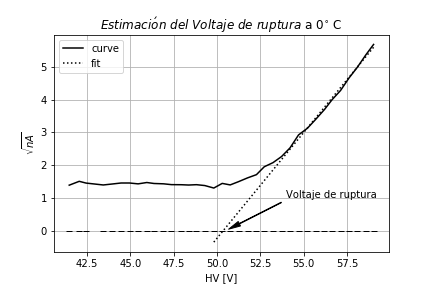
\includegraphics[width=0.7\textwidth]{cal_voltaje_ruptura.png}
\centering
\caption{Raíz cuadrada de la corriente oscura en función del voltaje de polarización a una temperatura de 0 $^\circ$C. El voltaje de ruptura es el punto de intersección entre el eje HV y la línea ajustada (fit) a la curva de la corriente oscura.} 
\label{voltaje_de_ruptura}
\end{figure}

Para estimar del voltaje de ruptura en cada una de las curvas, se utiliza un método que consiste en el cálculo de la raíz cuadrada de la corriente oscura en función del voltaje de polarización. Entonces el voltaje de ruptura es el punto intersección entre el eje del voltaje de polarización y la línea ajustada a la parte final de la curva como se muestra en la Fig.~\ref{voltaje_de_ruptura}. Este procedimiento se realizó para cada curva una de las curvas IV con el fin de obtener la gráfica del voltaje de ruptura en función de la temperatura, como se muestra en Fig.~\ref{voltaje_ruptura_vs_T}.\\


\begin{figure}[ht!]
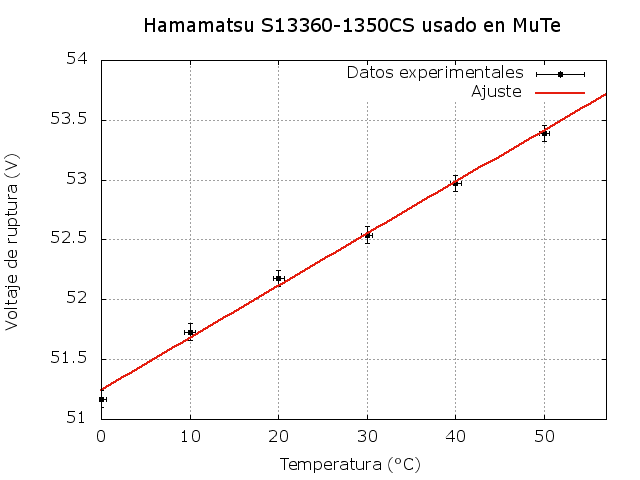
\includegraphics[width=0.7\textwidth]{voltajeRuptura.png}
\centering
\caption{Voltaje de ruptura en función de la temperatura para el SiPM S13360-1350CS.} 
\label{voltaje_ruptura_vs_T}
\end{figure}

\section{Conclusiones}
La implementación de un sistema de control de temperatura basado en dispositivos Peltier a partir de su modelo FOPDT permitió estudiar el voltaje de ruptura de los  SiPM S13360-1350CS que se utilizan en el telescopio de muones (MuTe). Dicho sistema de control logra estabilizarse a una temperatura objetivo en el rango de 0  a $50~^\circ$C en menos de 8 minutos.\\

Por otra parte, se obtuvo la curva característica IV del SiPM S13360-1350CS con el fin de obtener el voltaje de ruptura dependiendo de la temperatura entre 0 y $50~^\circ$C. Se observó como la corriente oscura del SiPM aumenta de forma exponencial luego que se supera el voltaje de ruptura, es decir, entra en la región de amplificación. Así mismo, se utilizó el método de la raíz cuadrada de la corriente oscura para estimar el valor del voltaje de ruptura y se encontró que la dependencia de la temperatura es 43 $mV/^\circ C$.\\

Finalmente, se determinó que para el rango de temperaturas a las que se va a someter el SiPM en el sitio de detección, el voltaje de ruptura varía desde los $51.5 $ V hasta $52.5$ V por lo tanto se debe garantizar la corrección del voltaje de polarización, el cual según el fabricante es el voltaje de ruptura más $3$ V~\cite{Sipm_S13360_1350CS_datasheet}.   %$0.043~\frac{^{\circ}C}{V}$

%  ---- Bibliography ----
% BibTeX users should specify bibliography style 'splncs04'.
% References will then be sorted and formatted in the correct style.
%
%\newpage
\bibliographystyle{splncs04}
%\bibliographystyle{unsrt}
\bibliography{Mendeley.bib}

\end{document}
